\documentclass[11pt]{article}
\usepackage[letterpaper,margin={1.5cm}]{geometry}
\usepackage[utf8]{inputenc}
\usepackage[T1]{fontenc}
\usepackage[spanish]{babel}
\title{\textbf{Reporte Final \\ Proyecto Baloto }}
\author{Eilin Luna Moreno\\
		Gisela Arrieta Rivera\\
			Yurani Melissa Palacios }
\date{}
\usepackage{graphicx}
\begin{document}

\maketitle

\section{Acerca de Baloto}

Baloto es un juego en línea en Colombia, que consiste en acertar en cualquier orden 6, 5, 4 o 3 números del 1 al 45.
 
Usted puede jugar a través de un tarjetón de juego que tiene 5 paneles para 5 apuestas distintas.
 
Baloto ofrece un acumulado inicial (ACUMULADO MULTIMILLONARIO) de 2.000 millones de pesos, el cual se irá acumulando cada sorteo si no es ganado, hasta poder entregarlo a un nuevo multimillonario.

\section{¿Es realmente aleatorio el Baloto?}
En el Baloto se espera que el comportamiento sea aleatorio y por ende la secuencia de mayor probabilidad no posee una significancia estadística. La idea del proyecto es la verificación de la aleatoriedad del Baloto.

\section{Etapas de desarrollo}
El desarrollo de este proyecto se realiza como una actividad de la clase Herramientas Computacionales de la carrera Computación Científica de la Universidad de Medellín de Colombia, siguiendo paso a paso las instrucciones dadas por el docente Edward Yesid Villegas.

\subsection{Etapa 1: Extracción y procesamiento}
La primera entrega tuvo como objetivo la creación de códigos que se encargaran de extraer datos web necesarios a partir de una fuente de datos externa. La figura 1 muestra la frecuencia de cada balota en la historia, cabe destacar que hay tantos datos devido a que se obtienen no solo los datos del baloto sino los datos del baloto revancha.


\subsection{Etapa 2: Estadística descriptiva}
La segunda entrega del proyecto de aula consistia en un avance de la etapa de análisis de datos. Haciendo un uso adecuado de funciones para el análisis estadistico inferencial y descriptivo, usando R y modulos de preferencia. Se realizó un calculo de la media, desviación estandar, máximo y mínimo (para cada sumatoria de las 6 balotas), además se hallaron dos secuencias, una de ellas contiene las seis frecuencias más repetidas, y la otra contiene las seis frecuencias que menos se repiten.

\
\subsection{Etapa 3: Estadística Inferencial}
\
La tercera y última entrega del proyecto de aula consistia en la finalización del proceso de análisis de datos, más la inclusión de gráficas de interés y el reporte final con el cual se analiza el cumplimiento o no del objetivo propuesto. Sin embargo lo máximo que alcanzamos a hacer fue hallar las diferencias que hay entre la frecuencia que más se repite y la que menos se repiten, siendo 64 la diferencia mayor, es decir, hay una diferencia de 64 sorteos de los 2042 (hasta el momento), siendo aproximadamente un tres por ciento del historico actual del Baloto, lo cual no es un porcentaje de gran significancia.
Además también se hallo el porcentaje de salida de cada balota, tendiendo a tener muy parecido porcentaje, lo cual desde ya podriamos ver que en definitiva el baloto sí es aleatorio, y si al menos existiera una mínima posibilidad de que fuera al azar, ésta pequeña probabilidad no tendría ninguna significancia, además influyen muchos más factores que no se tienen en cuenta (o se desconocen) para poder concluir con certeza que el baloto sea al azar. 

\begin{figure}[htp]
\centering
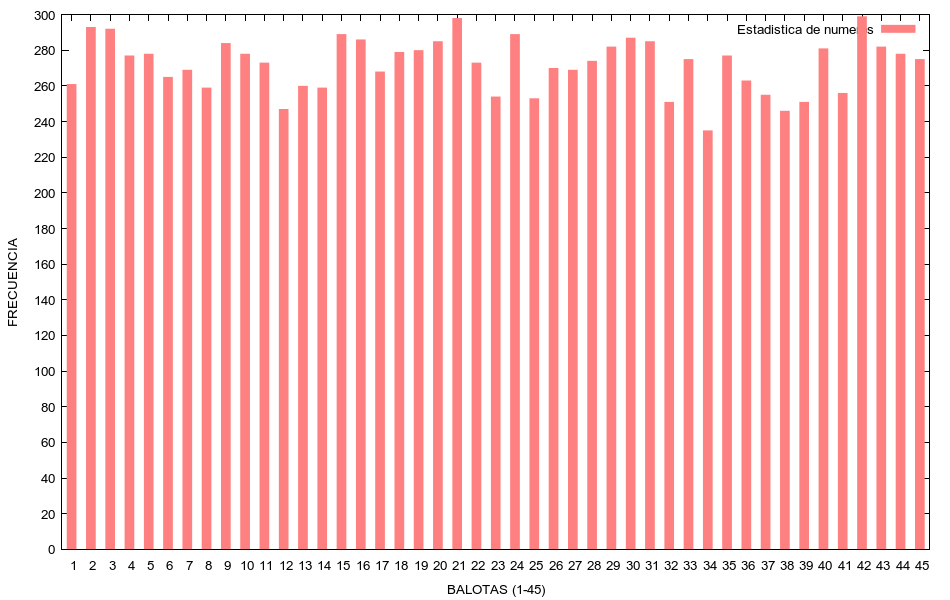
\includegraphics[scale=0.50]{/home/gia/Baloto/Codigo/Estadistica_de_numeros.png}
\caption{}
\label{}
\end{figure}

\end{document}